%!TEX root = ../thesis-guntur.tex
%************************************************
\chapter{Results}
\label{ch:results} % $\mathbb{ZNR}$
%************************************************
In this chapter, we report and summarize the result of the experiment presented in~\autoref{ch:experimental-setup}. The experiments try to investigate the correlation of social density level and smartphone sensor readings. We also investigate the behavior of \ac{MAC} address randomization that can potentially disrupt the data collection results. This chapter contains only important findings. We present the detailed findings in the Appendices.

We performed the experiment on October 2016. The results that we collected contain a total of 17,280 time-lapse images, 660 audio recording files, and 1,320 text-based log files. The sum of total file size is approximately 41,7 Gigabytes.

\section{MAC Address Randomization} % (fold)
\label{sec:mac-address-randomization}
We performed investigations of \ac{MAC} address randomization in iPad mini and Nexus 5X that run different mobile \ac{OS}, namely iOS and Android, respectively. We captured the probe request using Wireshark on MacBook Air laptop in remote area, where no other probe requests are observable. \autoref{tab:mac-address-randomization-summary}~summarizes the result of \ac{MAC} address randomization investigation using metrics that we mention in~\autoref{sec:mac_address_randomization}.

\begin{table}[ht]
\centering
\caption{Summarized result of \ac{MAC} address randomization behavior for both Android and iOS.}
\label{tab:mac-address-randomization-summary}
\begin{tabularx}{\textwidth}{lXX}
\toprule
                                        & iPad mini (iOS) & Nexus 5X (Android) \\
                                        \midrule
Timing    & broadcast in every 2 minutes & broadcast in every 1 minute \\ 
Variation & address changed in every 4 minutes & address changed in each probe request packet burst \\
\ac{SN} field & reset in each 2 probe request packet burst & no pattern observed \\ \bottomrule
\end{tabularx}
\end{table}

	\subsection{iPad mini} % (fold)
	\label{sub:ipad_mini}
	% when does the random mac appear?
	The iPad mini always transmitted randomized \ac{MAC} address when the screen is on and off (standby). However, the iPad broadcast the probe request packets more actively while the screen is on, as we noticed that the iPad mini was sending out probe request packets within 3 to 10 seconds in screen on condition. If the screen is off, the iPad mini sent out probe request packets approximately in every 2 minutes, or even 4 minutes. Interestingly, when the iPad was connected to an \ac{AP}, that we set up using Nexus 5X WiFi tethering, we observed the iPad mini's real \ac{MAC} address in the probe request.

	The randomized address was changed to completely different random address, i.e., all octets of the address, when the iPad mini woke up from standby mode. The address was also changed after roughly 4 minutes from the first random address transmitted. We also observed \ac{MAC} address change when we toggled the WiFi on and off. The iPad behaved in the same manner regardless of \ac{SIM} card installation. 

	\begin{figure}[h]
		\centering
		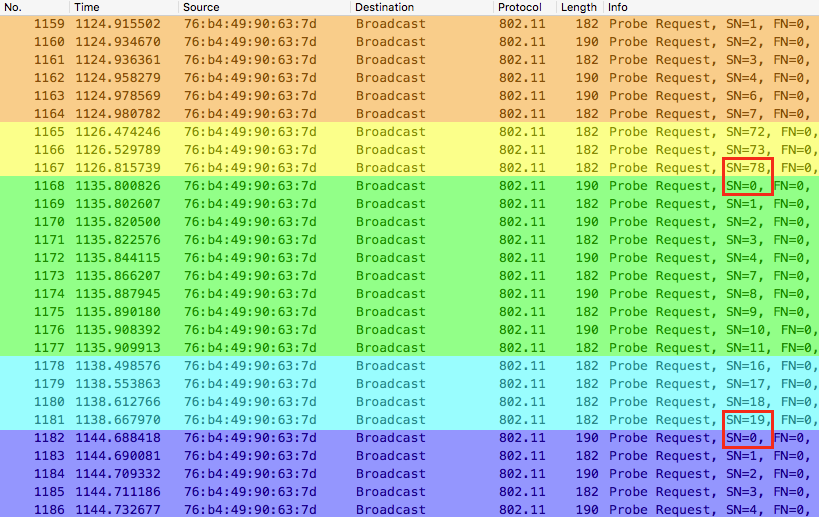
\includegraphics[width=\textwidth]{./img/result/randomization/ipad-mini}
		\caption[Some examples of captured probe requests from iPad mini.]{An example of captured probe requests from iPad mini in Wireshark. The colors mark out different bursts of probe request packets, while the red boxes indicate \ac{SN} reset.}
		\label{fig:ipad-random}
	\end{figure}

	% the SN
	\autoref{fig:ipad-random} depicts several examples of captured probe request packets from iPad mini, which were captured by Wireshark. The column represents, from left to right, the number of captured packet, the time of capture since beginning of capture (in second), the source address (\ac{MAC} address), the destination address, the communication protocol, packet length, and packet information.
	
	As we can see in~\autoref{fig:ipad-random}, the iPad mini reset the \ac{SN} after broadcasting two bursts of probe request. We can see in~\autoref{fig:ipad-random} that each burst, with nearly identical timestamp, is grouped in color. The red boxes mark the \ac{SN} reset, which mark a transition of \ac{SN} from 78 to 0, and 19 to 0.


	\subsection{Nexus 5X} % (fold)
	\label{sub:lg_nexus_5x}
	% when does the random mac appear?
	As opposed to iPad mini, Nexus 5X only sent out randomized \ac{MAC} address when the screen is off. If Nexus 5X woke up from sleep, it would immediately send out 4 or 10 probe request packets with real \ac{MAC} address. When Nexus 5X screen went off, Nexus 5X firstly sent out random \ac{MAC} address in every 2 to 10 seconds. Normally Nexus 5X broadcast a burst of probe request packets roughly in each 60 seconds.

	Unlike iPad mini, Nexus 5X changed the \ac{MAC} address in each burst of probe request packets, as depicted in~\autoref{fig:nexus-random}. However, the first three octets were always the same and only the last three octets were changed. We can see that \verb|da:a1:19| appears in multiple bursts in~\autoref{fig:nexus-random} with different last three octets, \verb|ce:47:5f|, \verb|00:3f:25|, and \verb|b5:51:2c|, respectively.
	
	\begin{figure}[h]
		\centering
		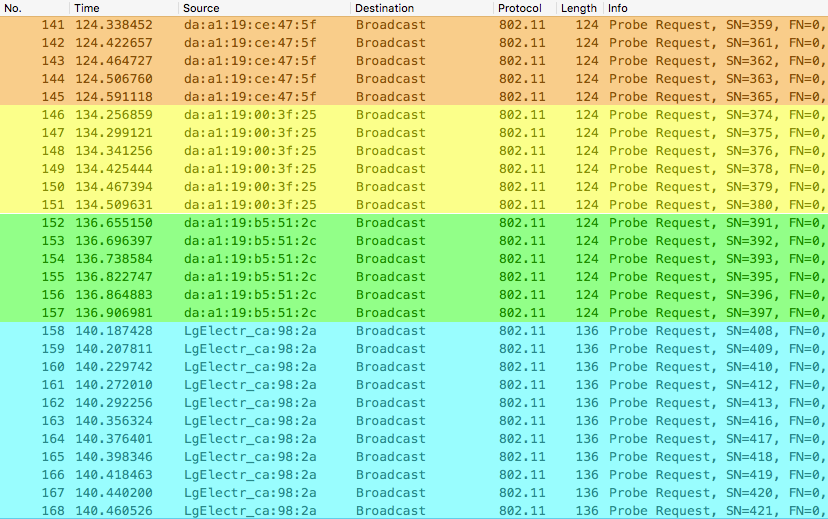
\includegraphics[width=\textwidth]{./img/result/randomization/nexus-5x}
		\caption[An example of captured probe requests from Nexus 5X.]{An example of captured probe requests from Nexus 5X in Wireshark. The colors mark out different bursts of probe request packets. The original \ac{MAC} address is indicated by cyan color in the last burst.}
		\label{fig:nexus-random}
	\end{figure}	

	% the SN
	\autoref{fig:nexus-random}~depicts example of captured probe request packets from Nexus 5X in the same format as~\autoref{fig:ipad-random}. There are four bursts of probe request packets marked in different colors. Three of the bursts are random \ac{MAC} address, while the last burst, marked in blue color, is the Nexus 5X original \ac{MAC} address.

	As we can see from~\autoref{fig:nexus-random}, the last probe request packet of a burst has a close \ac{SN} to the first packet of the next burst, although it is not sequential. We observed no pattern in \ac{SN} change during the experiment.

	\subsection{Review} % (fold)
	\label{sub:review}
	Based on our findings in \ac{MAC} address randomization investigation, to minimize the side-effect of randomized \ac{MAC} address in our final result, which could yield in counting the same device multiple times, we use 1 minute as the cycle length. This means we record ambient noise and capture time-lapse images within 1 minute time interval, while we capture probe request packets in 52 seconds followed by two times of \ac{AP} scanning (see~\autoref{sub:scanning}).


% maybe use this
% Use table of simulation about randomized mac address using different time window.

\section{Correlation between Crowd Count and Sensor Readings} % (fold)
\label{sec:crowd_count_correlation-result}
In this section, we present the result of data collection using 1 minute cycle length, which consist of probe request packet capture, \ac{AP} scan, ambient noise recording, and time-lapse images capture (see~\autoref{fig:sensor-measurement}). As for the ground truth estimation, we used head count of time-lapse images and device count in unique \ac{MAC} address in probe request. The result can indicate whether smartphone sensor readings can be an approach to estimate the level of social density or crowd count.

% when
We collected the data from Wednesday, October 26\textsuperscript{th} 2016, to Saturday, October 29\textsuperscript{th} 2016. The timing of data collection is shown in~\autoref{tab:location-summary}. During the data collection, we saw no special events where the social density level are more crowded than usual condition, especially in public places, such as Grote Markt and Paddepoel shopping center.

% assumption
In manual head counting, an object may appear more than once, i.e., the object was captured in multiple GoPro cameras, because we took time-lapse images and some people were actively moving. We used manual pattern recognition to avoid multiple counting. Furthermore, sometimes we captured vehicles in the images with very limited visual appearance of the people inside. Thus we assume that there are a person in a car and five people in a bus. We present some examples of time-lapse images in~\autoref{ch:appendix-time-lapse-images}.

\begin{figure}[h]
	\begin{adjustwidth}{-2cm}{}
	\centering
	\subfloat[head count]{
		\label{fig:population-head-count}{
			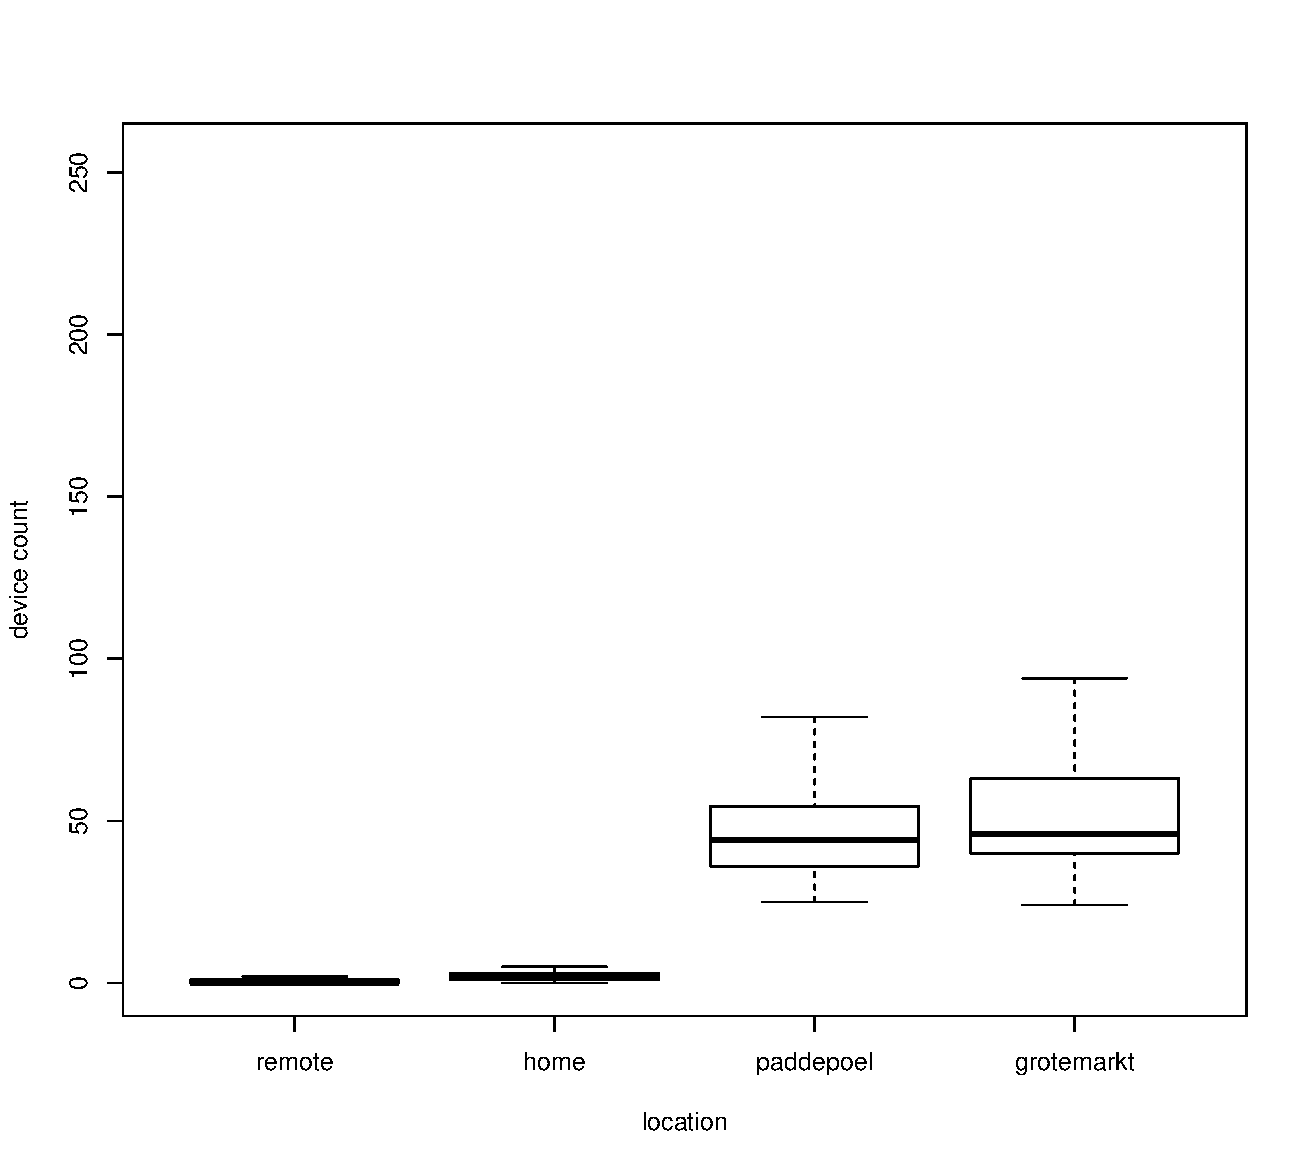
\includegraphics[width=0.65\textwidth]{./img/result/population-head-count}
		}
	}
	\subfloat[device count]{
		\label{fig:population-device-count}{
			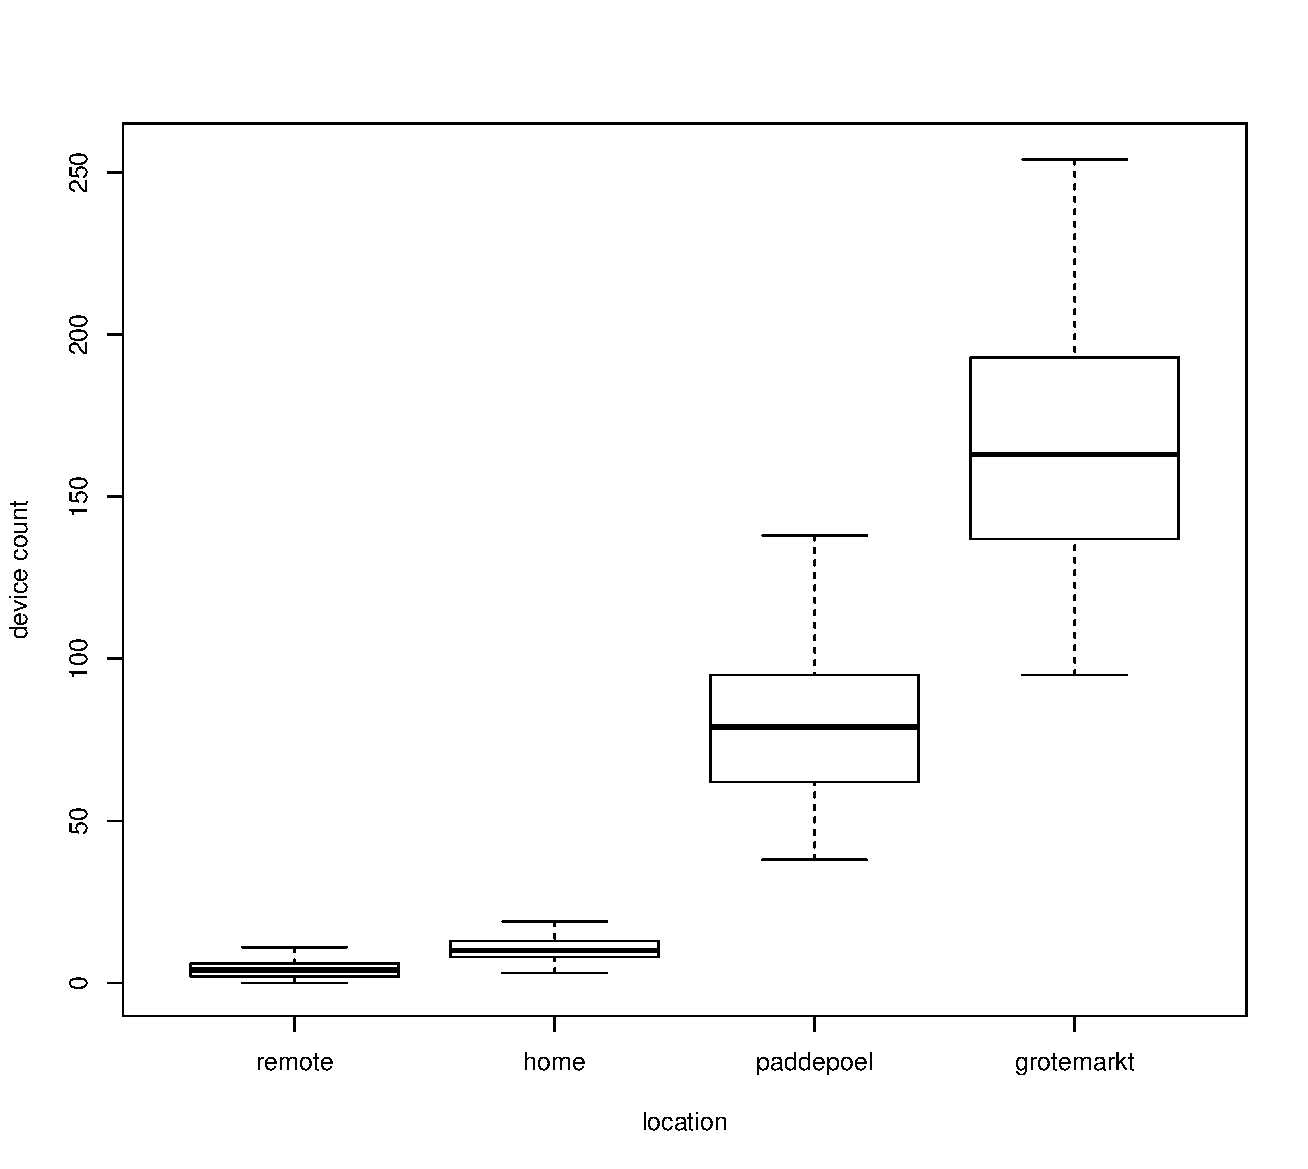
\includegraphics[width=0.65\textwidth]{./img/result/population-device-count}
		}
	}
	\end{adjustwidth}
	\caption{A box plot showing the population of estimated social density in each location by both head count (\ref{fig:population-head-count}) and device count (\ref{fig:population-device-count}).}
	\label{fig:total-population}
\end{figure}

Make the box plot to be more readable.

We present the important results of the experiment, such as the variation of the social density level, example of ambient noise recording, correlation of \ac{AP} count and sensor readings, the effect of scanning time, and all parameters used for analysis. The appendices present the detailed results, such as the sensor readings both in scatter plot and line chart (\autoref{ch:appendix-sensor-readings}), example of time-lapse images for each location (\autoref{ch:appendix-time-lapse-images}), and ambient noise recording (\autoref{ch:appendix-ambient-noise}).

\autoref{fig:total-population}~depicts the variation of estimated social density level in each location, e.g., the lowest value, the first quartile, the median, the upper quartile, and the maximum value. The value are estimated by two approximation, namely head count and device count.

As we can see in~\autoref{fig:total-population}, the maximum value of device count based estimation is higher than head count based estimation. For instance, in Grote Markt, the maximum value of device count is 288, while the maximum value of head count is 115. However, both estimations are showing the same trend, which says that Grote Markt has the highest social density level and remote area has the lowest social density level.

% device count
%    LOC Min  Q1 Med  Q3 Max
% 1:   r   0   2   4   6  11
% 2:   h   3   8  10  13  46
% 3:   p  38  62  79  95 150
% 4:   g  95 137 163 193 288

% head count
%    LOC Min Q1 Med   Q3 Max
% 1:   r   0  0   0  1.0   4
% 2:   h   0  1   2  3.0   5
% 3:   p  25 36  44 54.5  95
% 4:   g  24 40  46 63.0 115











	\subsection{Ambient Noise Recordings} % (fold)
	\label{sub:ambient_noise_recordings}
	As an example of ambient noise recording, \autoref{tab:ambient-noise-average-day4} and \autoref{fig:audio-result-day4} show the result of ambient noise recording in day 4. We measure the ambient noise in decibels (dB). In this unit, the closer the value to zero the louder the sound (noise). We take two measures of ambient noise to characterize the surrounding, namely the \ac{PKLV}, which is the highest value of a total waveform, and \ac{RMS}, which is the effective value or the mean of an audio recording. The \ac{PKLV} and \ac{RMS} are positively correlated but \ac{RMS} is more stable than \ac{PKLV}.

	\begin{table}[h]
	\centering
	\caption{The average of root-mean-square and peak level of ambient noise recording in day 4.}
	\label{tab:ambient-noise-average-day4}
	\begin{tabular}{lll}
	\toprule
	            & Root Mean Square (dB) & Peak Level (dB) \\ \midrule
	Remote area &  -47.74           &  -26.90          \\
	Home        &  -39.39         & -12.84          \\
	Paddepoel   & -26.54          &  -3.39        \\
	Grote markt & -36.29             & -5.87       \\ \bottomrule
	\end{tabular}
	\end{table}

	As we can see in the average value (\autoref{tab:ambient-noise-average-day4}) or line chart (\autoref{fig:audio-result-day4}), more crowded place has higher ambient noise value. We see that remote area is the quietest location, with -47.74 dB of average \ac{RMS}, while Paddepoel is the noisiest location, with -26.54 dB of average \ac{RMS}. As for the line chart, we can see more overlaps in \ac{PKLV} (\autoref{fig:peak-level-day4}) than in \ac{RMS} (\autoref{fig:rms-day4}). The \ac{RMS} of remote area is stable near -50.00 dB. We can also see the same trend for the rest of the ambient noise recordings although some overlaps are present, as shown in~\autoref{ch:appendix-ambient-noise}.
	

	\begin{figure}[H]
		% \centering
		\subfloat[peak level]{
			\label{fig:peak-level-day4}{
				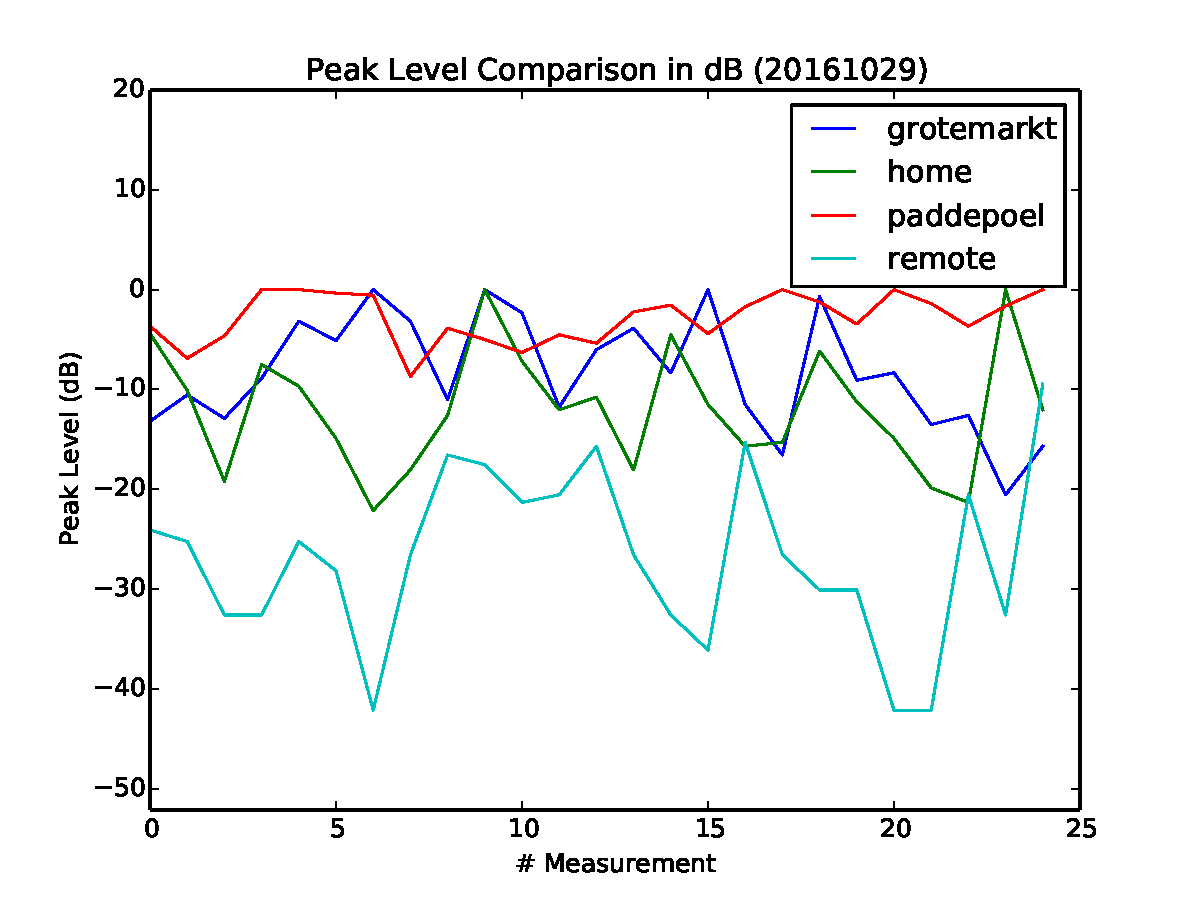
\includegraphics[width=0.8\textwidth]{./img/result/sound/peak-level-comparison-20161029}
			}
		}\\
		\subfloat[root mean square]{
			\label{fig:rms-day4}{
				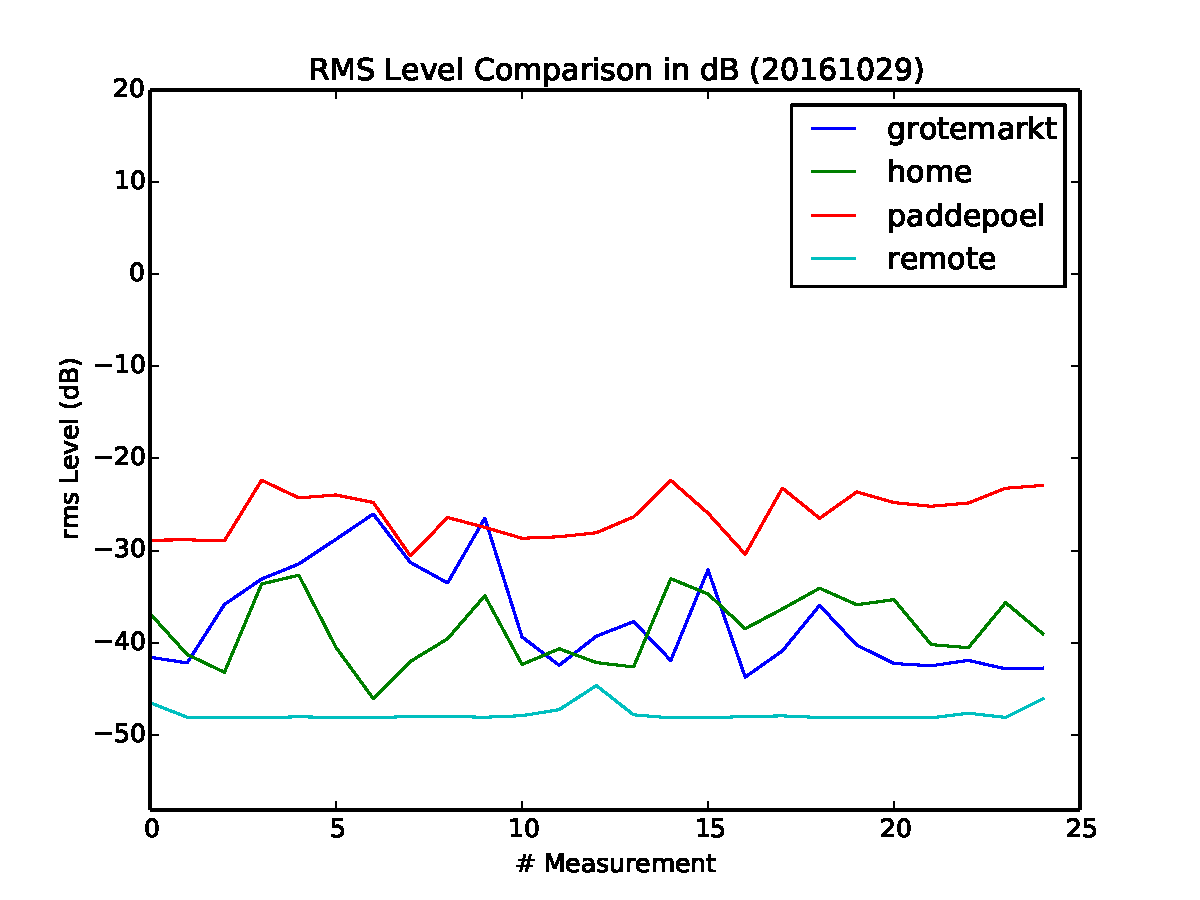
\includegraphics[width=0.8\textwidth]{./img/result/sound/rms-level-comparison20161029}
			}
		}
		\caption{Line chart showing the peak level (\ref{fig:peak-level-day4}) and root-mean-square (\ref{fig:rms-day4}) of the ambient noise recording in each cycle at day 4.}
	\label{fig:audio-result-day4}
	\end{figure}


	\subsubsection{Speaker Count Extraction} % (fold)
	\label{ssub:probe_request_based_estimation}
	In~\autoref{sec:line_charts}, we present the result of smartphone sensor readings that displays the estimated speaker count from ambient noise recording, extracted using unsupervised machine learning method by Xu, et al,~\cite{thesis067}. However, the result is not satisfying as the speaker count estimation is mostly yielding zero speaker count, even in the most crowded location. When we listened to the audio recording, sometimes human voice is present but not apparent and clear.

	To test the accuracy of unsupervised speaker count estimation from Xu, et al,~\cite{thesis067}, we apply the algorithm to audio recordings in which the speaker voice is apparent and clear. We select different audio recordings that have diverse speaker count, ranging from single speaker, as in a speech or monologue, two speakers, as in duets or interview, and five speakers, as in a cappella.

	We tune two parameters in the speaker count algorithm, namely ${\theta}_{s}$ and ${\theta}_{d}$, using recommended configuration in their implementation of the algorithm\footnote{\url{https://github.com/lendlice/crowdpp}}. The ${\theta}_{s}$ parameter refers to the confidence level that we can identify the same speaker, while ${\theta}_{d}$ is about new speaker. \autoref{tab:speaker-count-result} summarizes the result.

	\begin{table}[h]
	\begin{adjustwidth}{-2cm}{}
	\centering
	\caption{Speaker count result}
	\label{tab:speaker-count-result}
	\begin{tabular}{l|l|llllll}
	\toprule
	\multirow{2}{*}{Description} & \multirow{2}{*}{\specialcell{Total\\Speaker(s)}} & \multicolumn{6}{c}{Detected Speaker(s) (${\theta}_{s},{\theta}_{d}$)} \\
	                             &                                & (13, 18) & (14, 24) & (15.6, 21.6) & (16, 21) & (17, 22) & (18, 25) \\ \midrule
	speech                     & 1 & 11 & 5 & 6 & 7 & 6 & 5 \\
	monologue                    & 1 & 5 & 4 & 5 & 5 & 5 & 3 \\
	duets                        & 2 & 1 & 1 & 1 & 1 & 1 & 1 \\
	interview     			 & 2 & 5 & 5 & 5 & 5 & 5 & 5 \\
	a cappella                   & 5 & 5 & 4 & 4 & 4 & 4 & 4 \\
	\bottomrule 
	\end{tabular}
	\end{adjustwidth}
	\end{table}

	We can see from~\autoref{tab:speaker-count-result} that the speaker estimation is not accurate. The only accurate estimation is done using 13 and 18 as the ${\theta}_{s}$ and ${\theta}_{d}$, respectively, but it only applies to a cappella recording with five speakers. The estimation gives stable result for duets and interview recording along different combination of ${\theta}_{s}$ and ${\theta}_{d}$, although it is not correct. 







	\subsection{AP and Social Density Correlation} % (fold)
	\label{sub:ap_and_social_density_correlation}
	We are particularly interested in seeing the trend and correlation of \ac{AP} count and social density level, estimated by head count and device count. We draw a scatter plot of \ac{AP} count vs device count and \ac{AP} count vs head count separately, as well as device count vs head count to see the correlation of the two social density estimation. The plots are shown in~\autoref{fig:scatter-dc-ap}, \autoref{fig:scatter-hc-ap}, and \autoref{fig:scatter-hc-dc}. We also present the line chart of the readings in~\autoref{ch:appendix-sensor-readings}.

	\autoref{fig:scatter-dc-ap} depicts the correlation of device count and \ac{AP} count. The data plotted in~\autoref{fig:scatter-dc-ap} comes from all data combined from four days experiment. The location is coded in color so that we can distinguish which data comes from which location. The plots of the correlation separately in each day are also available in~\autoref{ch:appendix-sensor-readings}, shown in~\autoref{fig:ap-dc-scatterplot}.
	
	As we can see in~\autoref{fig:scatter-dc-ap} there is a positive trend that indicates both variable has a positive correlation. This means when the access point count increases, the device count, which points to social density level, increases as well. The correlation coefficient $\rho$ is 0.877, indicating a strong correlation, and the p-value is below 0.05, indicating that the result is significant. Each location forms a distinct cluster which is distinguishable. The cluster of home and remote are close and the cluster of Paddepoel and Grote Markt are adjacent. However, there is a gap that separates home-remote cluster and Paddepoel-Grote markt cluster.

	% all result - device count
	\begin{figure}[h]
		\centering
		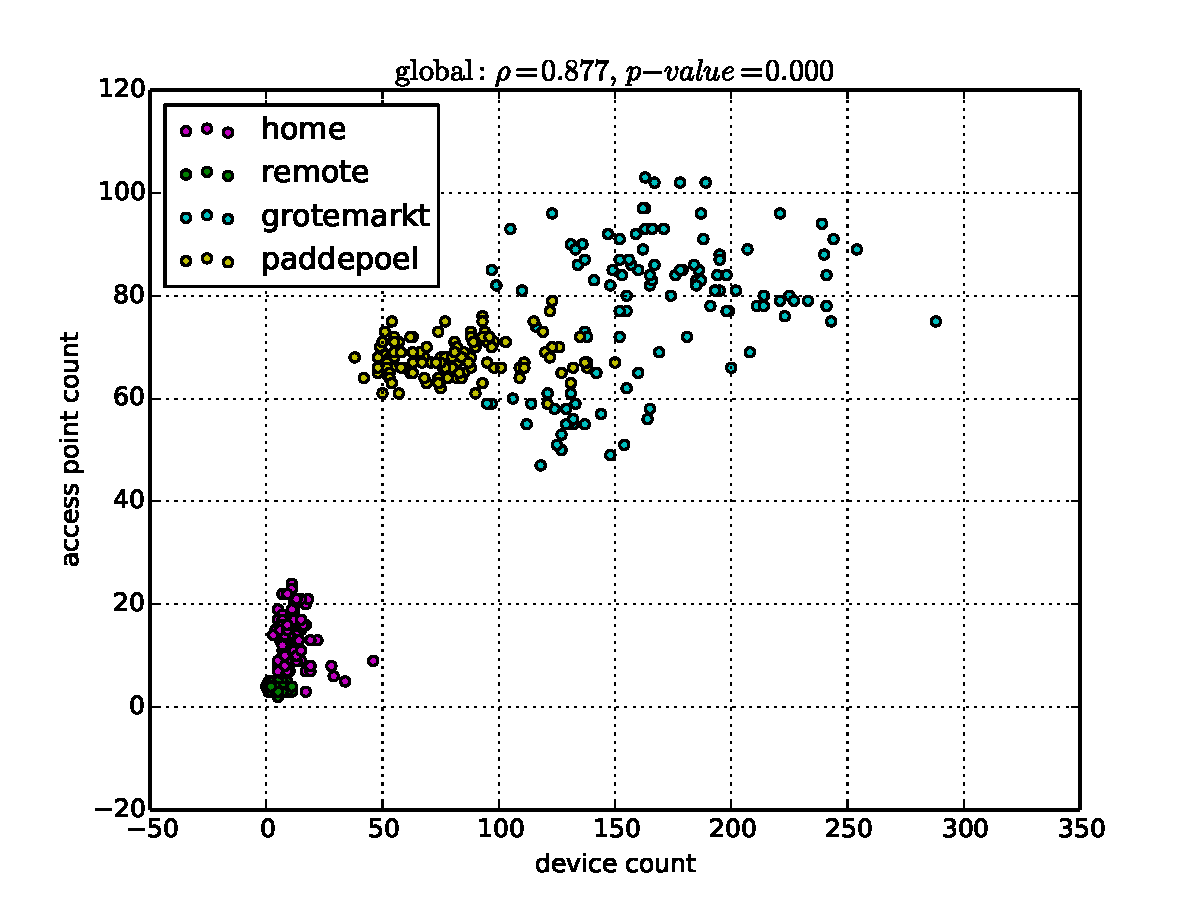
\includegraphics[width=0.8\textwidth]{./img/result/global-pr-vs-ap}
		\caption[Scatter plot showing the correlation of device count and \ac{AP} count.]
		{Scatter plot showing the correlation between \textit{device count} and \textit{\ac{AP} count} of all collected data. The locations are marked in different color. The correlation coefficient is $\rho=0.877$.}
		\label{fig:scatter-dc-ap}
	\end{figure}

	\autoref{fig:scatter-hc-ap} portrays the correlation between head count and \ac{AP} count of data collected in four days in all location. \autoref{fig:scatter-hc-ap} uses the same color coding as~\autoref{fig:scatter-dc-ap} to distinguish the location. The plots showing the correlation in separate days are available in~\autoref{ch:appendix-sensor-readings}, shown in~\autoref{fig:ap-hc-scatterplot}.
	
	We can see similar trend in~\autoref{fig:scatter-hc-ap}. The correlation is strong, indicated by correlation coefficient $\rho = 0.877$, and significant, indicated by p-value which is below 0.05. However, Grote Markt and Paddepoel clusters are overlapping. A gap between remote-home cluster and Grote Markt-Paddepoel cluster is also present.

	% all result - head count
	\begin{figure}[h]
		\centering
		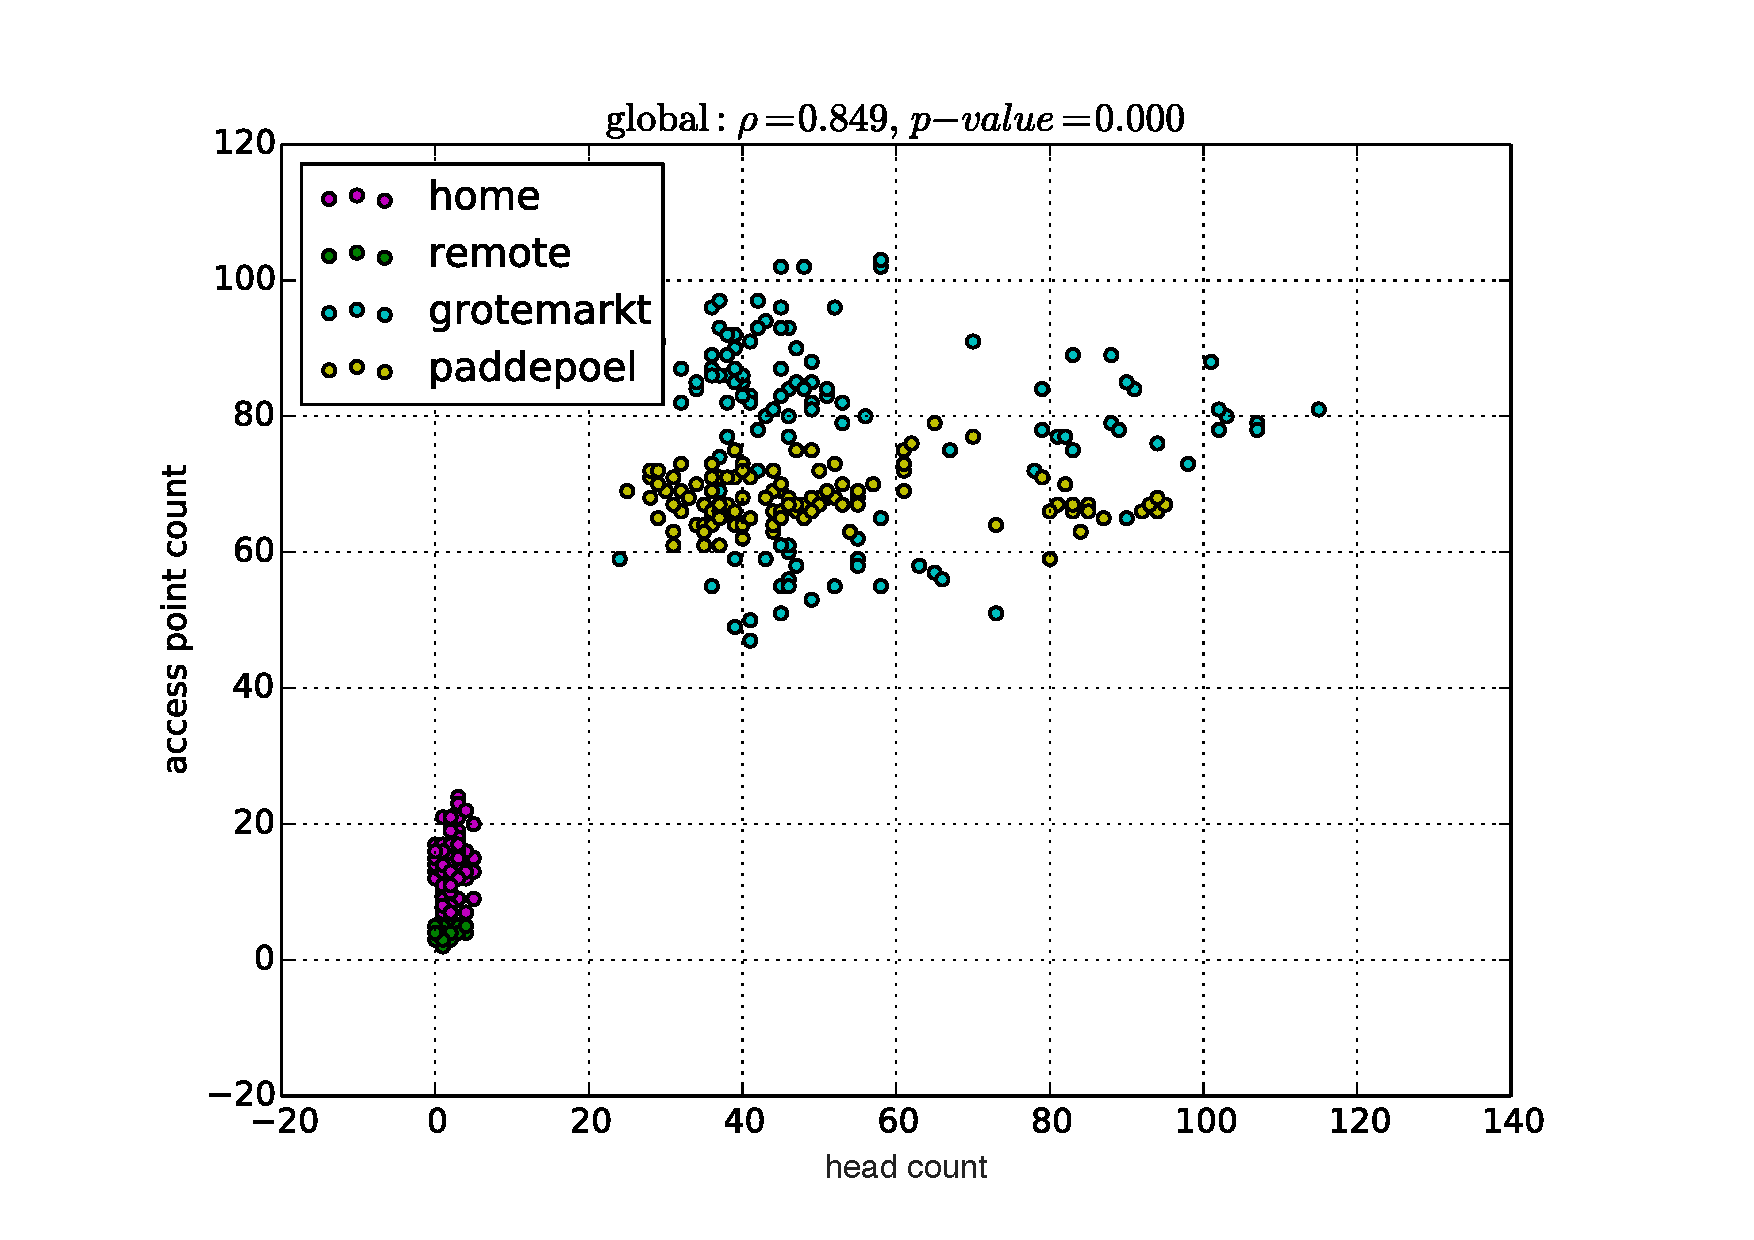
\includegraphics[width=0.8\textwidth]{./img/result/global-gt-vs-ap}
		\caption[Scatter plot showing the correlation of head count and \ac{AP} count.]
		{Scatter plot showing the correlation between \textit{head count} and \textit{\ac{AP} count} of all collected data. The locations are marked in different color. The correlation coefficient is $\rho=0.849$.}
		\label{fig:scatter-hc-ap}
	\end{figure}

	\autoref{fig:scatter-hc-dc} shows the correlation of head count and device count of all collected data. The locations are coded in color as well. Head count and device count have a strong correlation, marked by the correlation coefficient $\rho$, which is 0.857. A gap between remote-home cluster and Grote Markt-Paddepoel cluster is also present, although it is narrower than the gap in \autoref{fig:scatter-dc-ap} and \autoref{fig:scatter-hc-ap}. \autoref{fig:hc-dc-scatterplot} in \autoref{ch:appendix-sensor-readings} presents the scatter plots showing the correlation of head count and device count in each day of experiment.

	% all result - device count vs head count
	\begin{figure}[H]
		\centering
		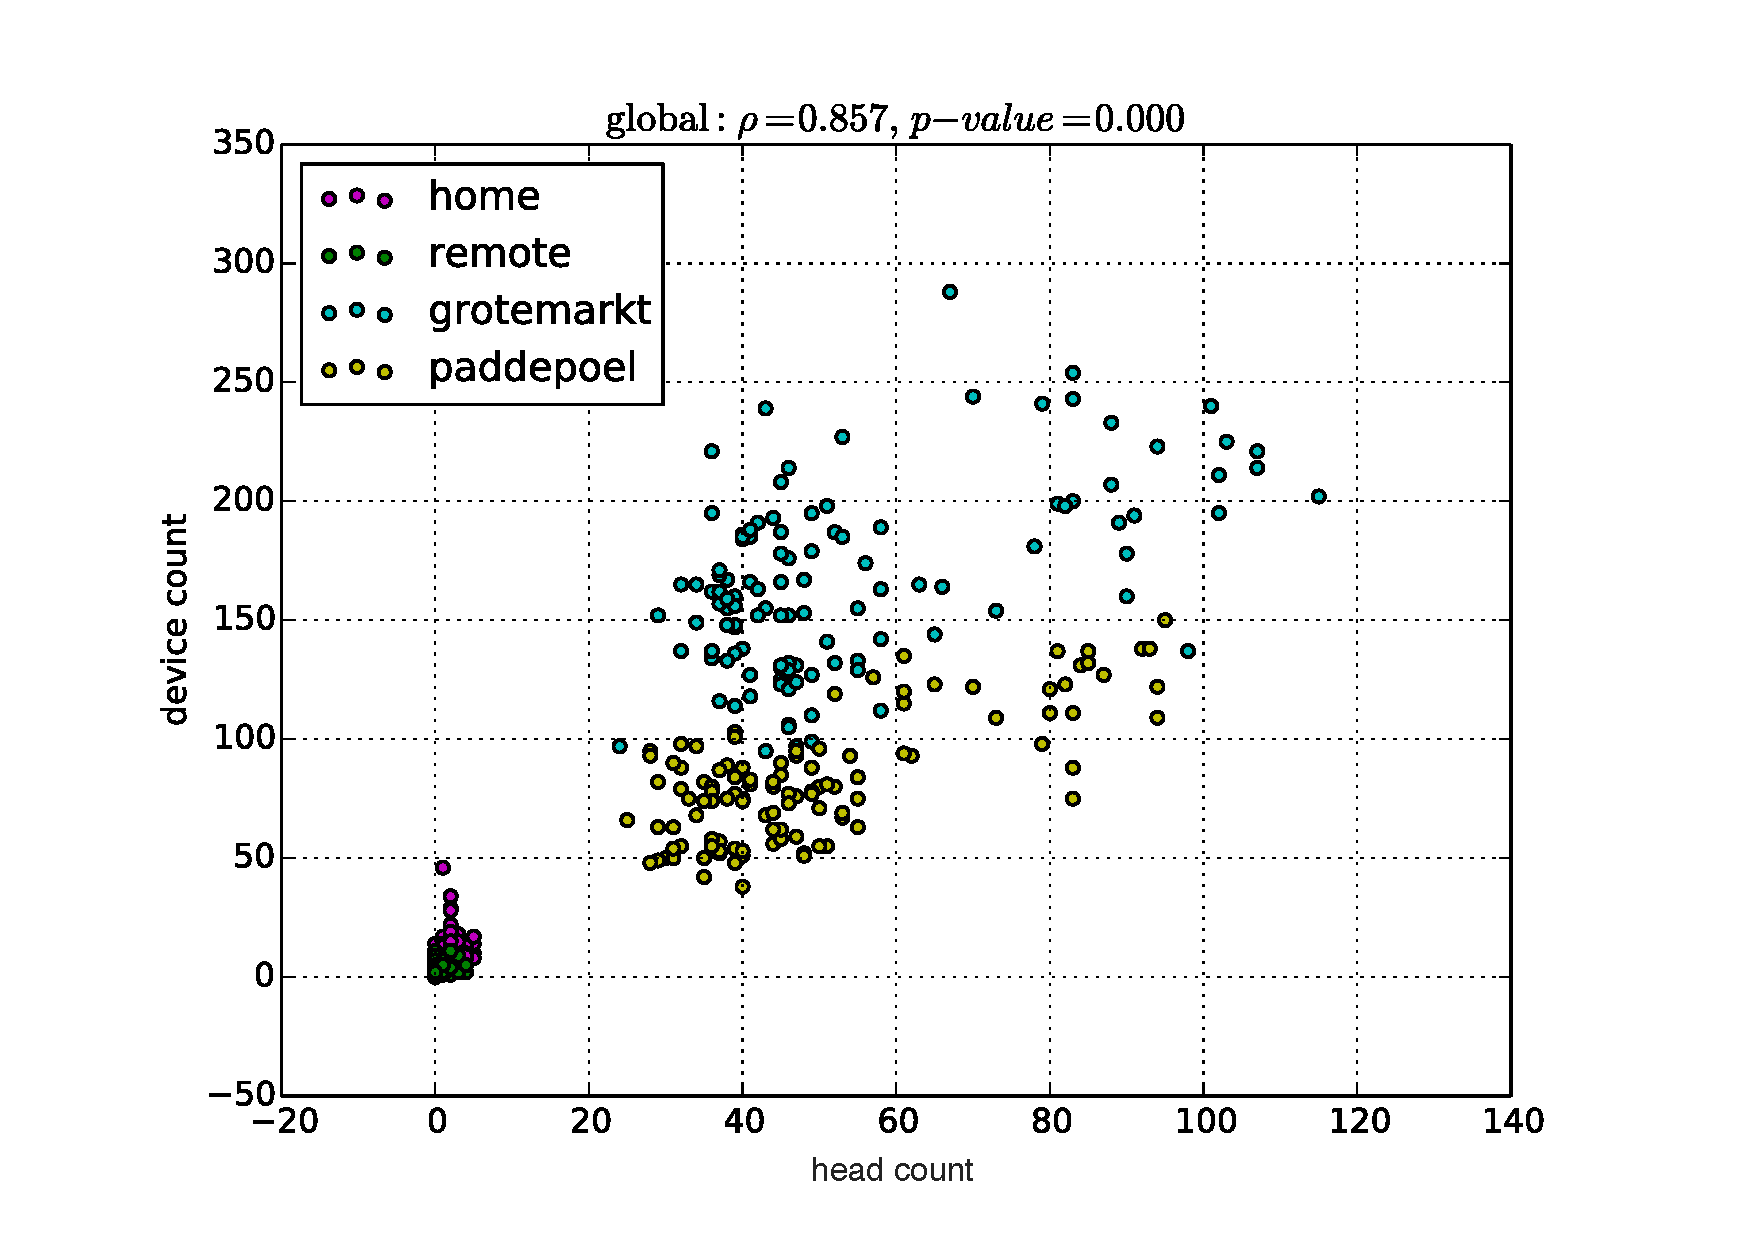
\includegraphics[width=0.8\textwidth]{./img/result/global-gt-vs-pr}
		\caption[Scatter plot showing the correlation of head count and device count.]
		{Scatter plot showing the correlation between \textit{head count} and \textit{device count} of all collected data. The locations are marked in different color. The correlation coefficient is $\rho=0.857$.}
		\label{fig:scatter-hc-dc}
	\end{figure}

	As we can see in three scatter plots (\autoref{fig:scatter-dc-ap}, \autoref{fig:scatter-hc-ap}, and \autoref{fig:scatter-hc-dc}), \ac{AP} and social density level from both head count and device count have a positive correlation. The correlation is strong, which is roughly 0.8 with p-value less than 0.05. 






	\subsection{Effect of Scanning Time} % (fold)
	\label{sub:effect_of_scanning_time}
	We performed four experiments on Sunday, October 30\textsuperscript{th} 2016, to investigate the effect of scanning time to the \ac{AP} count and social density correlation. We collected the data for 45 minutes, consisting WiFi and audio data, in four different time, namely
	\begin{enumerate*}[label={\alph*)},font={\color{red!50!black}\bfseries}]
	  \item 09:00,
	  \item 12:00,
	  \item 15:00,
	  \item and 18:00
	\end{enumerate*}.
	
	\autoref{fig:time-effect} shows the result in four separate line charts. Each chart depicts the result of a particular scanning time. The blue line, which depicts the \ac{AP} count, fluctuates stably around 100, while the green line, which represents device count, has a big variance. As we can see in~\autoref{fig:grotemarkt-0900}, the green line is fluctuating below the blue line, indicating there are less device than available \ac{AP} count. However, in~\autoref{fig:grotemarkt-1200}, \autoref{fig:grotemarkt-1500}, and \autoref{fig:grotemarkt-1800}, the condition changed. The green line surpasses the blue line, which indicates the number of device is increased. \autoref{fig:grotemarkt-1500} shows an increasing trend of device count, while \autoref{fig:grotemarkt-1800} shows a decreasing trend.

	\begin{figure}[h]
		\centering
		\begin{adjustwidth}{-1cm}{}
		\subfloat[09:00h]{
		  \label{fig:grotemarkt-0900}{
		    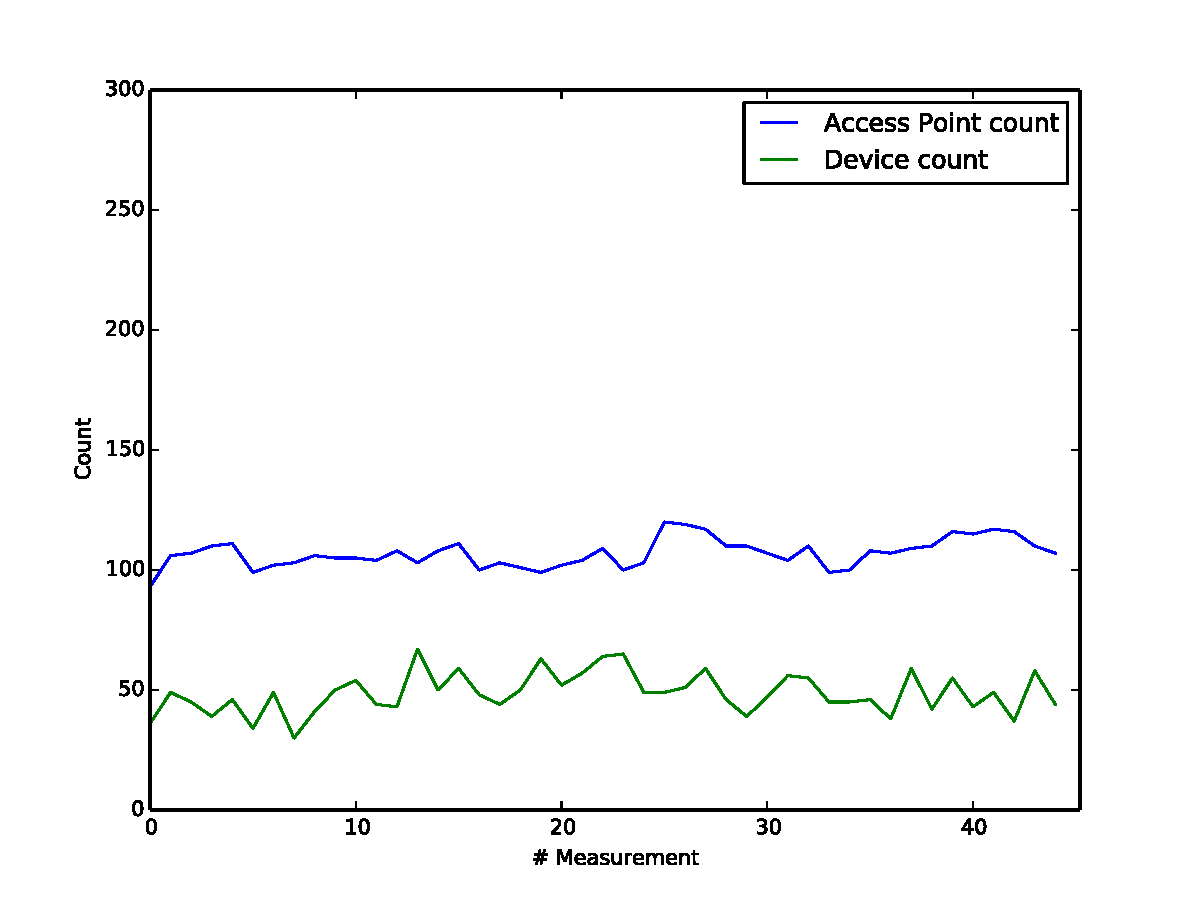
\includegraphics[width=0.7\textwidth]{./img/result/time/grotemarkt-0900}
		  }
		}
		\subfloat[12:00h]{
		  \label{fig:grotemarkt-1200}{
		    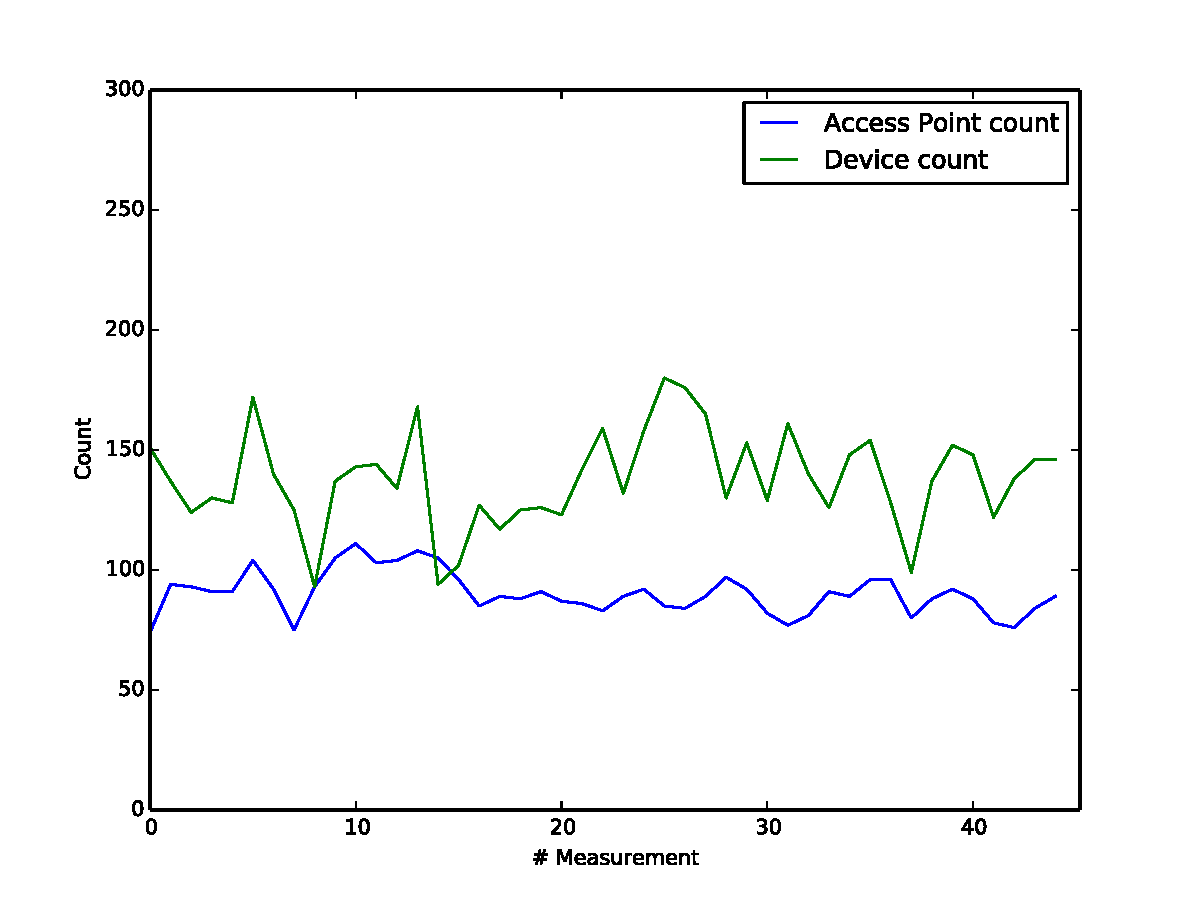
\includegraphics[width=0.7\textwidth]{./img/result/time/grotemarkt-1200}
		  }
		}\\
		\subfloat[15:00h]{
		  \label{fig:grotemarkt-1500}{
		    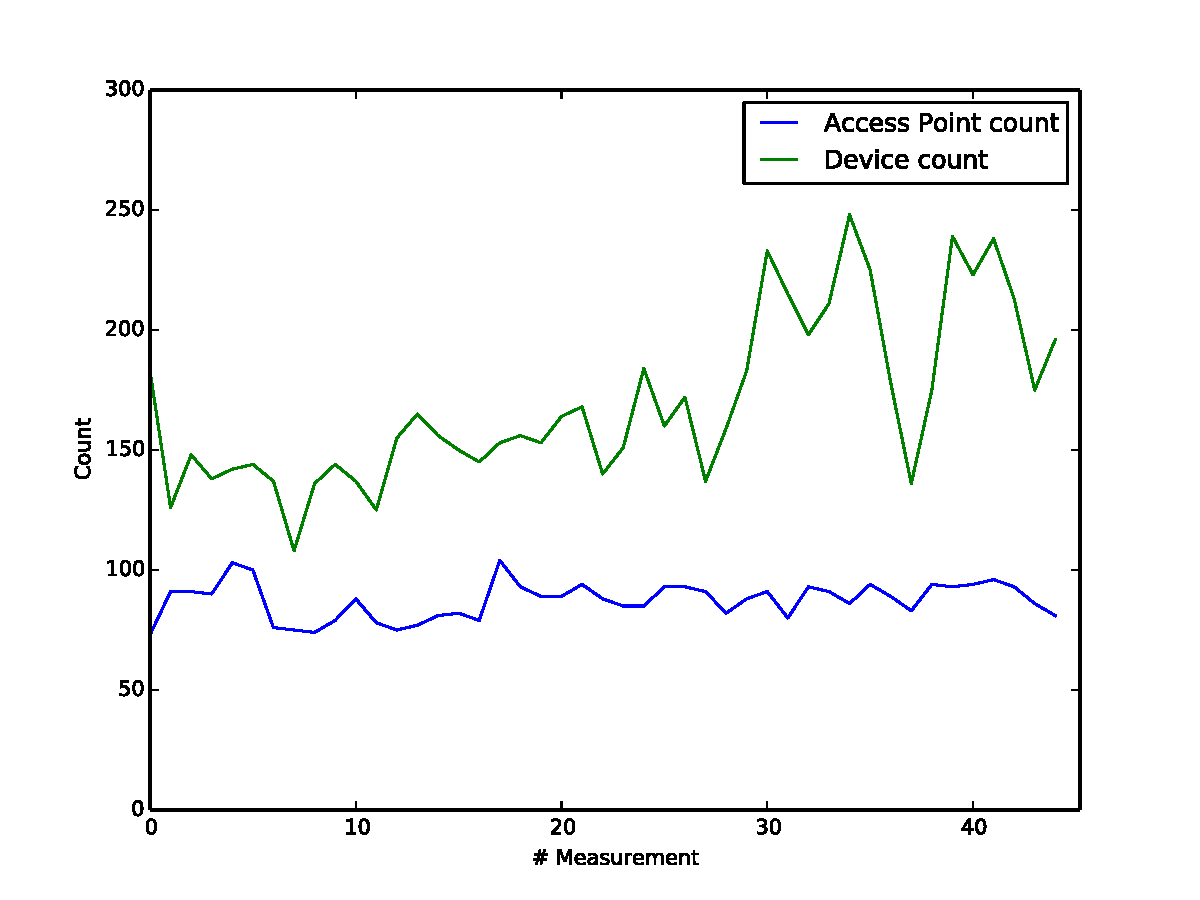
\includegraphics[width=0.7\textwidth]{./img/result/time/grotemarkt-1500}
		  }
		}
		\subfloat[18:00h]{
		  \label{fig:grotemarkt-1800}{
		    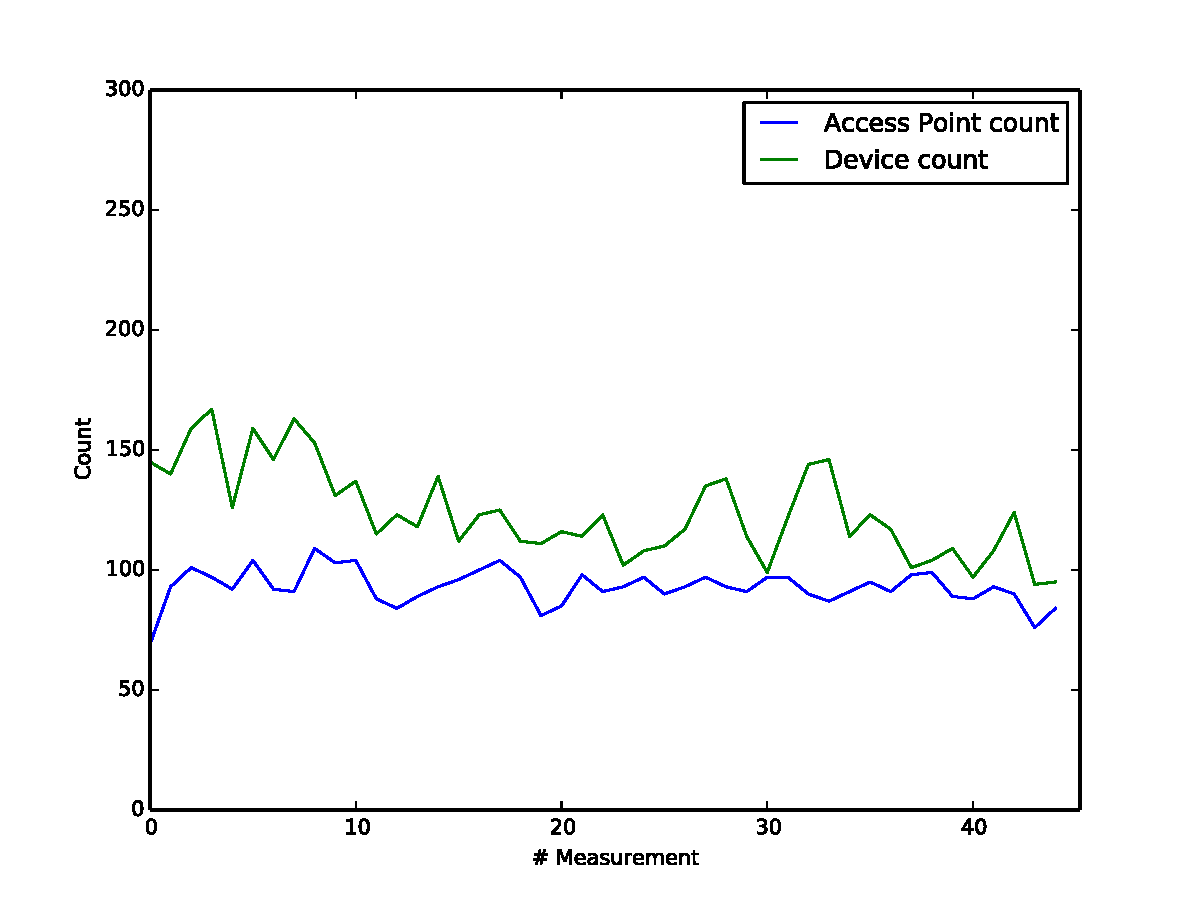
\includegraphics[width=0.7\textwidth]{./img/result/time/grotemarkt-1800}
		  }
		}
		\caption{Line charts showing the \ac{AP} count (blue) and device count (green) in different data collection time at Grote Markt, Groningen, at October 30, 2016.}
		\label{fig:time-effect}
		\end{adjustwidth}
	\end{figure}









	\subsection{All Result} % (fold)
	\label{sub:all_result}
	\autoref{fig:scatterplot-matrix} shows all data collected in four days of experiment in a scatter plot matrix. In the lower left part are the scatter plots of each parameter correlation along with the Lowess curve fitted to the data. In the upper part are the correlation coefficient and the p-value. Along the diagonal are the histograms and the labels of each parameter.

	There are eight parameters extracted from all datasets of four days experiment. \ac{AP}, \ac{RSSI}, \ac{DC}, and \ac{SNR} parameters are from WiFi based readings. \ac{AP} is the count of available \ac{AP} that a smartphone can get, while \ac{RSSI} is the average of the signal strength of the \ac{AP}. \ac{DC} is the device count, based on unique \ac{MAC} address, and \ac{SNR} is the average of signal-to-noise ratio of the captured probe request packets. \ac{SC}, \ac{RMS}, and \ac{PKLV} are from recorded ambient noise, while \ac{HC} is from manual head counting of time-lapse images.

	\begin{figure}[h]
		\begin{adjustwidth}{-3cm}{}
		\centering
		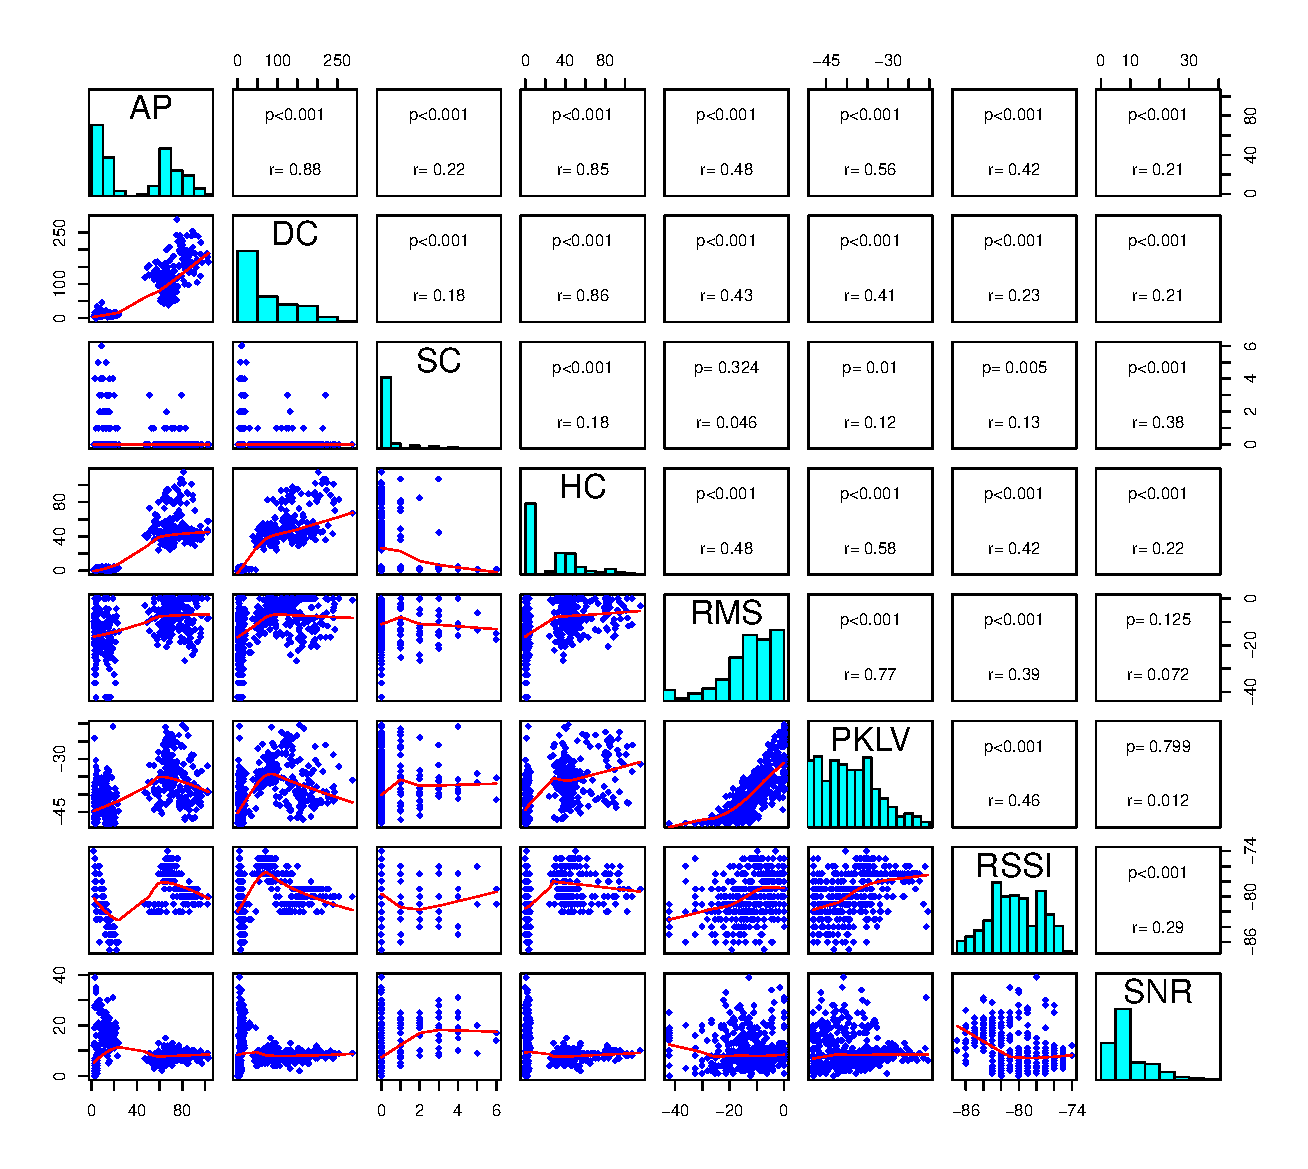
\includegraphics[width=1.3\textwidth]{./img/result/all-result}
		\end{adjustwidth}
		\caption[Scatter plot matrix showing all parameters correlation.]
		{Scatter plot matrix showing all parameters correlation of all collected data. The top right shows the correlation coefficient $r$ and the p-value. Along the diagonal are the histograms of each parameter.}
		\label{fig:scatterplot-matrix}
	\end{figure}

	In the next chapter, we present regression analysis about social level density estimation using all data from four days experiment. The regression analysis tries to simulate the social density estimation using consumer smartphone sensor readings.

	We predict the head count or device count from other parameters, e.g., \ac{AP}, \ac{RMS}, \ac{PKLV}, and \ac{RSSI}. We do not use \ac{SC} as a predicting variable because speaker count value is almost at zero, which does not give us any meaningful insight, and we do not use \ac{SNR} parameter as well, because we derive signal to noise ratio from probe request packet capture in a laptop, which smartphone cannot capture.

% Make the datasets available online.
% Make sure that the data is available publicly, mention the url.
%*****************************************
%*****************************************
%*****************************************
%*****************************************
%*****************************************
